\documentclass[12pt, a4paper]{report}
    \usepackage[T1]{fontenc}
    \usepackage[utf8]{inputenc}
    \usepackage{pdfpages}
    \usepackage{float}
    \usepackage{listings}
    \usepackage{siunitx}   
    \usepackage{nicefrac}
    \usepackage{pifont}
    \usepackage{xcolor}
    \usepackage[toc]{glossaries}
    \makeglossaries
    \newglossaryentry{Rolling shutter}
    {
      name=Rolling shutter,
      description={When the camera needs to capture an image, it reads out pixels from the sensor a row at a time rather than capturing all pixel values at once}
    }
    
    \newglossaryentry{Balance wheel}
    {
      name=Balance wheel,
      description={is a wheel that regulates or stabilizes the motion of a mechanical watch and is responsible for the clock to run precisely}
    }
    
  \newglossaryentry{Time scale}
    {
      name=Time scale,
      description={is used to measure the rate deviation of a mechanical watch in different positions}
    }
    
    \newglossaryentry{SAD}
    {
      name=SAD,
      description={(sum of absolute differences) is a positive number, which results from the formation of the difference between two digital images. It serves as a measure of the difference between two images and is used in image processing and pattern recognition. It is obtained by subtracting the color values of the images pixel by pixel from each other and adding them up by amount}
    }
    
    \newglossaryentry{MMAL}
    {
      name=MMAL,
      description={(Multimedia Abstraction Layer) is a framework designed by Broadcom to provide a host-side, simple and relatively low-level interface to multimedia components running on the Videocore IV GPU on the Raspberry Pi}
    }
    
    \newglossaryentry{Optical flow}
    {
      name=Optical flow,
      description={The optical flow of an image sequence is the vector field of the velocity projected into the image from visible points of the object in the reference system of the imaging optics}
    }
    
    \newglossaryentry{Codecvisa}
    {
      name=Codecvisa,
      description={CodecVisa is a powerful real-time analyzer for different video codecs. http://www.codecian.com/}
    }
    
  \newglossaryentry{VCHI}
    {
      name=VCHI,
      description={}
    }
    
  \newglossaryentry{API}
    {
      name=API,
      description={}
    }
    
      \newglossaryentry{DMA}
    {
      name=DMA,
      description={(Direct Memory Access) allows specific hardware systems of a computer system to access main system memory independently of the CPU \cite{Kuck1978}}
    }
    
          \newglossaryentry{CPU}
    {
      name=CPU,
      description={(Central Processing Unit) is the electronic circuitry in a computer, which executes the instructions of a computer program. \cite{Kuck1978}}
    }
    
   \newglossaryentry{Photon}
    {
      name=Photon,
      description={is an elementary particle, which includes electromagnetic radiation (e.g. light) and moves at the speed of light within a vacuum. \cite{Halliday2005}}
    }

    \newglossaryentry{Motion blur}
    {
      name=Motion blur,
      description={Motion blur is the apparent streaking of rapidly moving objects in a still image or a sequence of images such as a movie or animation.}
    }

    
    
    
    
    \usepackage{booktabs}
    \usepackage{float}
    \usepackage{hyperref}
    \usepackage{mathtools}
    \hypersetup{
        colorlinks,
        citecolor=black,
        filecolor=black,
        linkcolor=black,
        urlcolor=black
    }
    
    \usepackage{tabularx}
        \newcolumntype{L}{>{\raggedright\arraybackslash}X}
     
     \usepackage[style=numeric, backend=biber]{biblatex}
     \bibliography{PA_cogsworth_citation}

     
    \begin{document}
    
    \begin{titlepage}
    
    \newcommand{\HRule}{\rule{\linewidth}{0.5mm}} % Defines a new command for the horizontal lines, change thickness here
    
    \center % Center everything on the page
    
    \textsc{\LARGE ZHAW School of Engineering}\\[1.5cm] % Name of your university/college
    \textsc{\Large Projektarbeit}\\[0.5cm] % Major heading such as course name
    \textsc{\large IT}\\[0.5cm] % Minor heading such as course title
    
    \HRule \\[0.4cm]
    { \huge \bfseries Measurement of Rate Deviation}\\[0.4cm] % Title of your document
      { \huge \bfseries  of Watches with Raspberry Pi Camera}\\[0.4cm] % Title of your document

    \HRule \\[1.5cm]
    
    
    \begin{minipage}{0.4\textwidth}
    \begin{flushleft} \large
    \emph{Authors:}\\
    Linda Helen \textsc{Boedi}  Valentin \textsc{Bossi} % Your name
    \end{flushleft}
    \end{minipage}
    ~
    \begin{minipage}{0.4\textwidth}
    \begin{flushright} \large
    \emph{Supervisor:} \\
    Hans-Joachim  \textsc{Gelke} % Supervisor's Name
    \end{flushright}
    \end{minipage}\\[2cm]
    
    
    {\large \today}\\[2cm] 
    
    
\includegraphics[scale=0.05]{Images/logo.png}\\[1cm] 
    
    \vfill 
    
    \end{titlepage}
    
    \pagenumbering{roman}
    
    \chapter*{Declaration of Autonomy}
     \addcontentsline{toc}{chapter}{Declaration of Autonomy}
     
     The undersigned certify with their signature that the work has been written independently and put into written form, that the involvement of other persons has been limited to consulting and proofreading, and that all documents and guarantors used are listed.

 \vskip4cm
$\overline{\hbox{\phantom{mmmm}Place and Date\phantom{mmmm}}}$\hskip2cm
$\overline{\hbox{\phantom{mmm}Linda Helen Bödi\phantom{mmm}}}$

\vskip3cm
$\overline{\hbox{\phantom{mmmm}Place and Date\phantom{mmmm}}}$\hskip2cm
$\overline{\hbox{\phantom{mmmm}Valentin Bossi\phantom{mmmm}}}$

\chapter*{Abstract}
 \addcontentsline{toc}{chapter}{Abstract}
Every mechanical watch must be checked for accuracy both during manufacture and use. Most of the equipment used for this purpose is expensive. In this work it is determined whether a Raspberry Pi and a Raspberry Pi camera can be turned into a cheaper measuring device that can compete with the accuracy of a professional device. This camera also differs from conventional measuring devices in the type of measurement. Almost all devices on the market perform acoustic measurements and a few complement this measurement with an optical measurement by means of a laser beam. In this work a new approach is used; the measurement is carried out completely optically, but without laser beam, but completely by means of image processing. 
\newline
The following questions should be clarified in the work: Is a complete optical measurement by means of image processing possible? How accurate will these measurements be and can they keep up with the results of professional equipment? What are possible sources of error? How can the measurement be further improved? 
\newline
In a first step, possible methods were then evaluated in order to carry out the optical measurement of the frequency of the balance wheel of a watch. A closer look was taken at the OpenCV library, the gstreamer, a one-to-one comparison of images, tracking a specific pixel and the Picamera library. Since the Picamera library has a very well-founded documentation and offers many of the functionalities needed for this work, the decision was made in the end for this library. In order to better understand the motion vectors, various experiments were carried out, whereby the camera settings were also improved. After this basis had been established, a first rough calculation of the frequency was done by hand in Excel and due to a promising result the implementation of a Python program was carried out. During the work, after several measurements with professional instruments, it was found that the watch reacts very sensitively to temperatures, runs very inaccurately and therefore it is difficult to get good reference measurements. Therefore, a comparison was made with a blinking LED which flashes in time to show how the test clock should ideally oscillate back and forth. The measurements of the flashing LED showed that the determination of the frequency by means of image processing works very well and that sufficient good results can be achieved. In order to improve the results even further, it is possible, for example, to investigate which camera settings are best suited for the measurement. 
Overall the measurements with the camera are a little bit worse than those with professional devices, but it is not impossible to get a similar accuracy when some error sources are eliminated (e.g. by testing out other and maybe better camera settings and better light conditions).

\pagebreak
    \setcounter{secnumdepth}{5} 
    \setcounter{tocdepth}{5} 
    \pagenumbering{gobble}
    \tableofcontents
    \pagebreak
    \pagenumbering{arabic}
    
    \chapter{Motivation}
    Today's watch technology requires measuring instruments to perform a wide variety of measurements and analyses on almost all types of watches with great precision and reliability.
    Mechanical watches must be checked in production and service for their rate deviation.
    There are different techniques to measure this deviation; on one hand acoustically and optically or only acoustically.
    The aim of this work is to develop a handy device that can visually measure the rate deviation using inexpensive and simple means.
    To achieve this, an existing camera consisting of the best-known single-board computer Raspberry Pi and the corresponding camera from Raspberry Pi is used.
    The aim of this work is to use image processing to measure and analyse the rate deviation of mechanical clocks.
    The vision of this project is to be able to perform real-time measurements as established providers do with a much cheaper device.
    
    \chapter{Fundamentals}
    This chapter is intended to lay the foundation for this report. An overview of the existing measuring methods for the accuracy of a mechanical watch is given and the Raspberry Pi camera, which was used for the optical measurements in this project, is described. In addition, the functionality of a mechanical watch is explained and important information about the test watch is listed.
    \section{Competitor Analysis}
    At the beginning a small historical excursion, or rather an overview of the existing measuring methods for the accuracy of a mechanical watch.
     \subsection{Optical versus acoustical measurement}
    To measure the frequency of the balance wheel of a mechanic clock there exist mainly two methods on the market; acoustical and optical measurement. The common used method is by analyzing the beat noises of the lever escapement. More expensive devices use both acoustical and optical feedback. In order to be able to classify the rate deviation well enough, it is usually measured in different positions of the watch.
    
    \subsubsection{Acoustical measurement}
    The first used method to get the frequency measurement of the balance wheel was by using a vibrograph. For every "tick" of the clock a line was drawn onto a ongoing strip of paper. Out of the distance between of these lines the frequency was calculated \cite{Zeitwaage}. But as this method isn't the most accurate other techniques are used nowadays.  
    Modern watch timing machines use an oscillating quartz crystal as comparison for the frequency of the balance wheel \cite{Zeitwaage}. The beat noises of the lever escapement are recorded and amplified with a microphone whereat unwanted background noises need to be filtered out. 
    
    \subsubsection{Optical measurement}
    About hundred years later, optical watch timing machines joined the acoustical ones. There are barely devices on the market, which use only optical measurement, but several companies started to combine their acoustical with optical metering. One way to scale the frequency of the balance wheel optically is by using a laser. The beam will be periodically interrupted by the balance wheel and thus the frequency can be calculated \cite{Lombardi2011}. In this paper the frequency should be quantified optically by using image processing. There is hardly to none company out there, which uses the last technique for measuring the frequency.
    
        \begin{table}[H]
     \centering
    \begin{tabularx}{\linewidth}{ |c||L|L|  }
     \hline
     \multicolumn{3}{|c|}{\textbf{Comparison acoustical and optical measurement}} \\
     \hline
     & \textbf{acoustical}  & \textbf{optical} \\\hline
      since   &  around 19th century (2)  & end of 20th century (2)\\ \hline
     accuracy &   0.1 s/d & 0.1 s/d\\  \hline
     advantages & - most experience (exists for about 200 years) \newline - tracks if balance wheel is damaged (different noises) & measurement can be done anywhere\\  \hline
     disadvantages & background noises need to be filtered out&laser needs to be positioned precisely \\
     \hline
    \end{tabularx}
    \caption{Comparison of acoustical and optical measurement}
        \end{table}
        
    
    \subsection{Companies}
     In the following section the three largest companies producing such measuring instruments are described and the most important facts listed.
    \subsubsection{Witschi - WisioScope S}
    WisioScope S tests mechanical watches acoustically and optically. The measurement is done parallel and in this way is more accurate as both signals are used for the calculation of the frequency.
    The optical metering is done using a laser and lighting, a camera helps to adjust the watch properly. The costs of their product are: CHF 10450.-
    
    \subsubsection{Lepsi - WatchScope/WatchAnalyzer}
    The WatchScope and WatchAnalyzer from Lepsi are especially for watch lovers and not really for production. Both products are Swiss technologies. Both devices only work with an acoustic input, with measurements of either a few seconds or up to 24 hours. All data can then be queried with the smartphone. WatchScope is the smaller, more convenient version. With the WatchAnalyzer you can easily measure the rate deviation of the watch in several positions. The prices for this product are CHF 369.00, resp. CHF 929.-
    
    
    \subsubsection{Greiner Vibrograf - Compact 900}
    The Compact 900 measures only the beat noises of the ever escapement. The price is CHF 4070.-
    
    \bigskip
   The following table summarizes all important information for the three mentioned professional devices.
    
\begin{table}[H]
     \centering
    \begin{tabularx}{\linewidth}{ |c||L|L|L|  }
     \hline
     \multicolumn{4}{|c|}{\textbf{Measurement rate deviation}} \\
     \hline
     &{\fontsize{9}{10}\selectfont \textbf{Witschi - WisioScope S}}  & {\fontsize{8}{9}\selectfont \textbf{Lepsi - WatchScope/WatchAnalyzer} }& {\fontsize{9}{10}\selectfont \textbf{Greiner Vibrograf - Compact 900} }\\\hline
      Scope   &  +/- 999.9 s/d  & +/- 1000 s/d &  +/- 1000 s/d \\ \hline
     Resolution &   0.1 s/d & 0.1 s/d & 0.1 s/d\\  \hline
     Price & CHF 10450.- & CHF 369.-, resp. CHF 929.- &  CHF 4070.-\\  \hline
    \end{tabularx}
    \caption{ Measurement rate deviation with different professional devices}
 \end{table}
    
    \section{Camera module}
    The documentation for the picamera library \cite{ReadTheDocsPicamera} provides a good introduction to the operation of the Raspberry Pi with camera, which is used for all measurements in this project. This chapter will briefly summarize this introduction to better understand the hardware and operation of the Raspberry Pi camera.
    
    The camera module of the Raspberry Pi is basically a mobile phone camera module. Among other things, it uses a rolling shutter to take pictures. The pixel values of a frame are not captured completely at once, but are read line by line.
    
    However, the sensor is configured via the registers with the number of lines to be read and a corresponding time. The sensor reads the lines and pushes the data with the configured speed to the Raspberry Pi.
    
    This keeps the readout time of each line constant. However, the CPU does not speak directly to the camera, but the processing rather takes place on the GPU (VideoCore IV) of the Raspberry Pi, which operates its own real-time operating system (VCOS).
    
    \bigskip
    \noindent
    \begin{figure}[H]
    \centering
    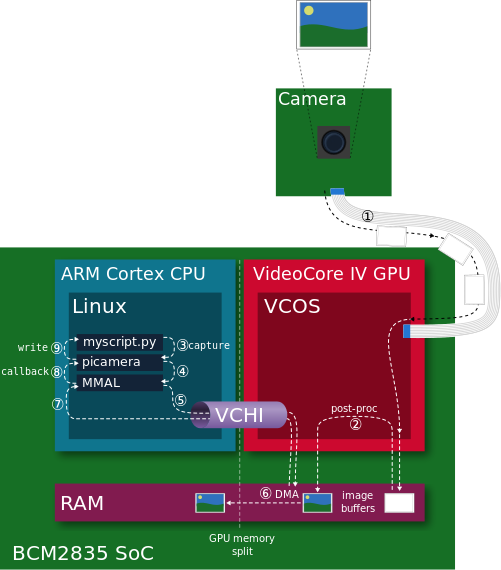
\includegraphics[scale=0.7]{Images/camera_architecture.png}
    
    \caption{Camera architecture. \cite{ReadTheDocsPicamera}}
    \end{figure}
    
    
    
    \bigskip
    
    The illustration above illustrates the processing flow of a frame, with the associated steps explained in the following section.
    
    \begin{enumerate}
    \item The camera's sensor is configured and continuously streams frame lines to the GPU.
    \item The GPU builds complete frame buffers from these lines and performs the post-processing of these buffers.
    \item Meanwhile, myscript.py makes a capture call with the picamera on the CPU.
    \item The picamera library uses the MMAL API to meet this requirement.
    \item The MMAL API sends a message via VCHI requesting a frame capture.
    \item The GPU then initiates a DMA transmission of the next full frame from its RAM portion to the CPU portion.
    \item Finally, the GPU sends back a message via VCHI that the capture is complete.
    \item This causes an MMAL thread to trigger a callback in the picamera library, which in turn retrieves the frame.
    \item Last picamera calls "write" on the output object provided by myscript.py.
    \end{enumerate}
    
    \subsection{Exposure time}
    
    The camera sensor detects how many photons hit the sensor elements, because the more impact, the more they increase their counter values. The sensor can perform exactly two operations; reset a set of elements or read a set of elements.
    
    \subsubsection{Minimal exposure time}
    
    Reading out a series of elements takes a certain amount of time, thus there is a limit to the minimum exposure time. Assuming one has 500 lines on a sensor and reading each line takes at least 20ns, then it will take at least $500*20 \text{ns} = 10 \text{ms}$ to read a full screen. 
    
    \subsubsection{Maximum framerate}
    
    The frame rate is the number of frames the camera can capture per second. The exposure time determines the maximum number of images that can be taken in a given time. Assuming it takes 10ms to read a complete image, then no more than $\frac{1 \text{s} }{10 \text{ms}} = \frac{1\text{s}}{0.01\text{s}} = 100 $ images in one second. 
    
    \bigskip
    
    So it is valid: 
    \begin{displaymath}
    \frac{1\text{s}}{\text{min exposure time in s}} = \text{max framerate in
    fps.} 
    \end{displaymath}
    The lower the minimum exposure time, the higher the maximum frame rate and vice versa.
    
    \subsubsection{Maximum exposure time}
    To maximize shutter speed, the framerate needs to be reduced. 
       \newline
      
        \bigskip
    Therefore the following is valid :
    \begin{displaymath}
    \frac{1\text{s}}{\text{min framerate in fps}} = \text{max exposure time
    in s}
    \end{displaymath} 
    
    \subsection{Hardware limits}
    
    \begin{itemize}
    \item The picamera originally has a very limited zoom to record the watch properly a lens was added to the camera in this project.
    \item The maximum horizontal resolution for the standard H264 recording is 1920 (this is a limitation of the H264 block in the GPU).
    \item The maximum frame rate of the camera depends on several factors. With overclocking 120fps can be achieved, but 90fps is the maximum supported frame rate.
    
    \end{itemize}
    
    
    \section{Mechanical watches}  
    In the following, the function of a mechanical watch is explained in more detail and the role of a watch's balance wheel is explained. Subsequently, important information on mechanical watches, such as the duration of stroke and facts about the test watch used in this project, are described.
    \subsection{Operation of a mechanical watch}  
    If a mechanical watch is wound up over the crown, the locking wheel (3) is moved by the winding shaft (1) and winding wheels (2). It turns the spring core (4) and pulls the tension spring in the mainspring barrel (5). The spring transmits the stored energy via the external toothed mainspring barrel (5) to the minute wheel (6), third wheel (7) and fourth wheel (8). 
    \newline
    \noindent
    \begin{figure}[H]
    \centering
    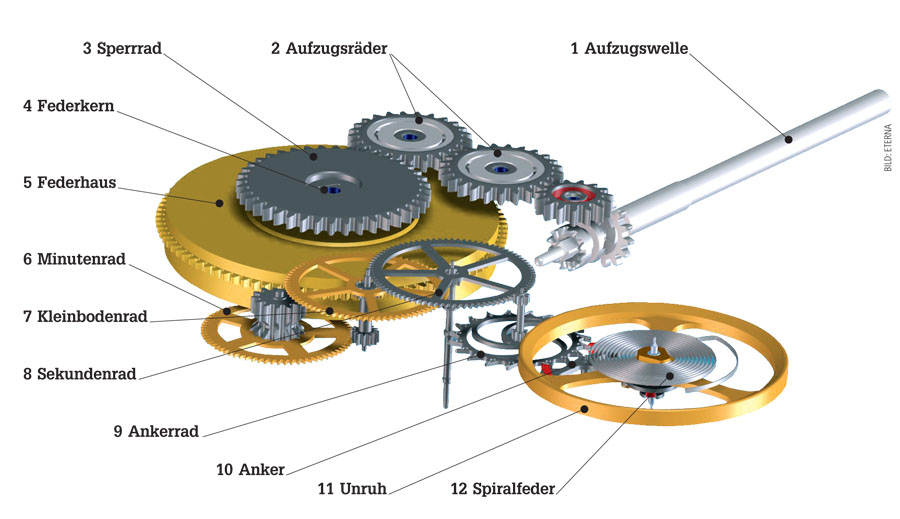
\includegraphics[scale=0.45]{Images/Funktionsweise-Uhrwerk.jpg}
    
    \caption{Operation of a mechanical watch \cite{Uhrwerk}}
    \end{figure}
The so-called escapement ensures that the gear train runs at the correct speed. The fourth wheel (8) drives the escape wheel (9); it gives an impulse to the pallet fork (10) which it passes on to the balance wheel (11), after which the armature, which moves back and forth like a seesaw, blocks the escape wheel. The balance wheel rotates, but is then retracted by the hairspring (12). It moves the armature back, which now releases the armature wheel again a little bit, which gives the armature with its rotation the next impulse. Due to the sudden braking and acceleration of the escapement wheel, the second hand of a mechanical watch also moves stepwise. \cite{Uhrwerk}
    \newline
    \noindent
    \begin{figure}[H]
    \centering
    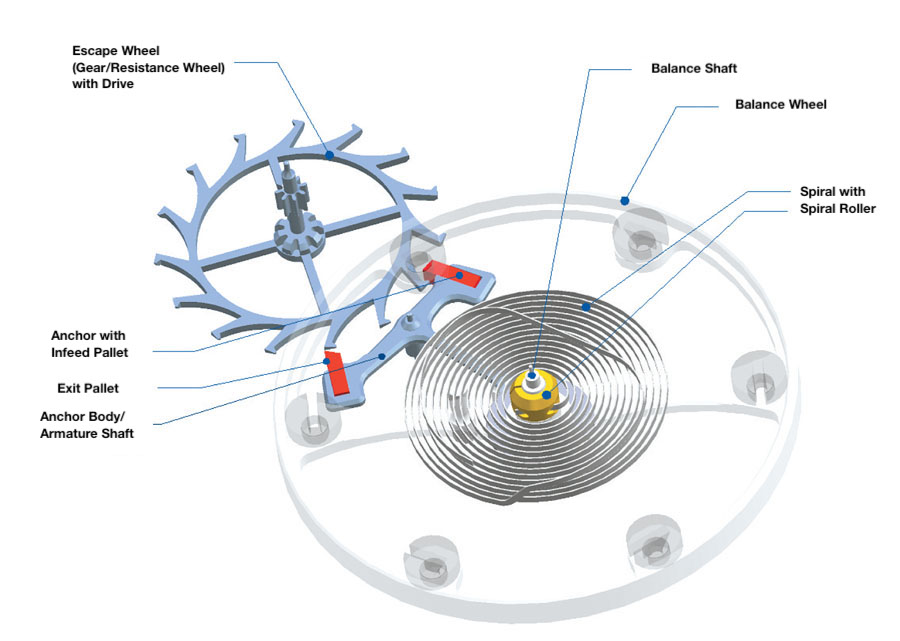
\includegraphics[scale=0.45]{Images/Hemmung-Teil1.jpg}
    
    \caption{Lever escapement and balance wheel \cite{Uhrwerk}}
    \end{figure}
\bigskip
The balance wheel is the heart of the oscillation system. It generates a time-defined movement, which in turn is transferred to the gear train and passed on to the watch hands. 
The occurring error, if the balance wheel does not run accurate, is called rate deviation. The deviation can be caused by different external and internal matters. Internal motives often are wear, resp. erosion or dirt. Whereas there are a lot more external causes as changes in temperature, air pressure or magnetism.

\subsection{Oscillation of the balance wheel}
In the following section the movement of the balance wheel, which will be recorded and used for the calculation of the frequency, is explained.

\subsubsection{Period}
The period of the balance wheel is the path of a point from one turning point to the other and back (A - B - A). \cite{Witschi_basics}
    \begin{figure}[H]
    \centering
    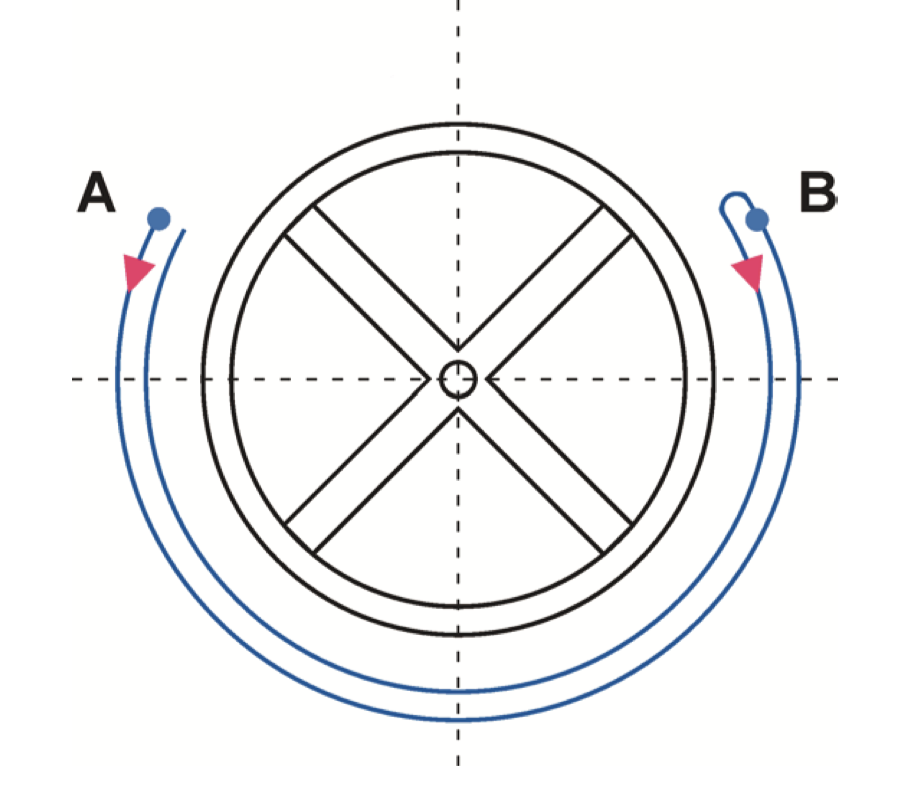
\includegraphics[scale=0.4]{Images/period.png}
    
    \caption{Period of the balance wheel \cite{Witschi_basics}}
    \end{figure}
\bigskip

\subsubsection{Half a period}
Half of a period, resp. one stroke, of the balance wheel is the path of a point from one turning point to the other (A - B). \cite{Witschi_basics}
    \begin{figure}[H]
    \centering
    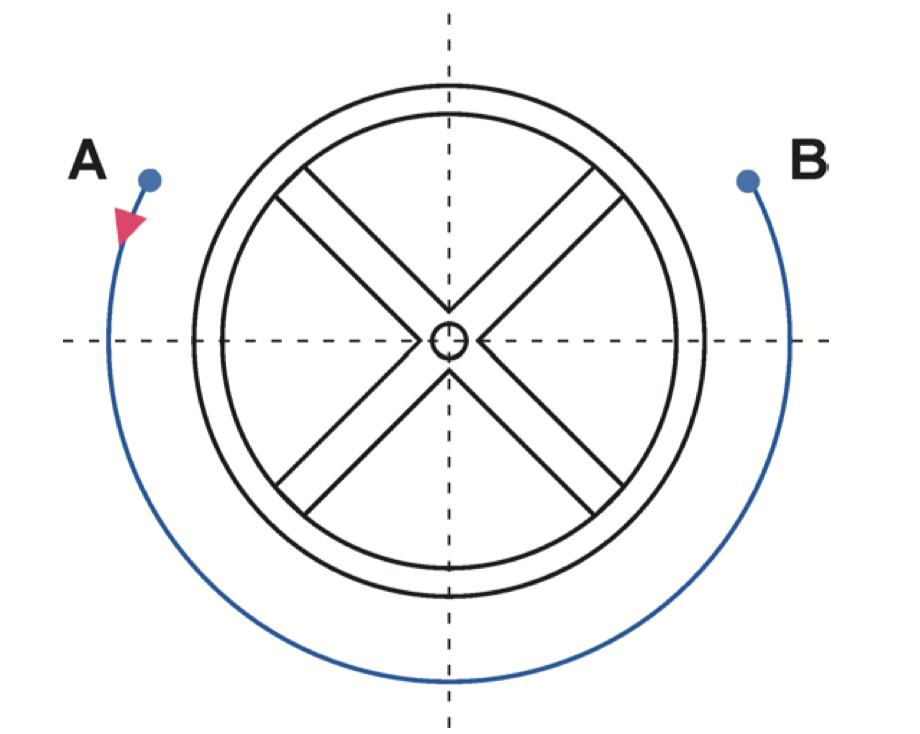
\includegraphics[scale=0.4]{Images/Halfperiod.png}
    
    \caption{half of a period of the balance wheel \cite{Witschi_basics}}
    \end{figure}
\bigskip
    
    \subsection{Number of strokes}
    Since the rate deviation has been calculated in seconds per day and the number of strokes per hour, i. e. the number of audible impulses of a two-armed pallet fork of a mechanical watch per hour, is known, these two quantities must first be brought to a unit. The relationship between the number of strokes (n*) and frequency (f) is as follows \cite{Krug1987}: 
    
    \begin{displaymath}
    n\text{*} = 2f*3600
     \end{displaymath}
     and therefore:
     \begin{displaymath}
      f = \frac{n\text{*}}{7200}
     \end{displaymath}
     
     \bigskip
     
    The following table lists facts about mechanical wristwatches. Among other things, it contains the number of strokes per hour, the duration for one stroke - i. e. half a period - and the frequency.
    
     \begin{table}[H]
     \centering
    \begin{tabularx}{\linewidth}{ |L|L|L|L|L|  }
     \hline
     \textbf{Number of strokes} [1/h] &  \textbf{Stroke duration} [s]& \textbf{Oscillation number}  [1/h]& \textbf{Period duration} [s]& \textbf{Frequency} [Hz]\\\hline
      18'000   &  0.200  & 9'000 & 0.400 & 2.50\\ \hline
     19'800 &  0.182 & 9'900 & 0.364 & 2.74\\  \hline
     21'600 &  0.166 & 10'800 & 0.333 & 3.00\\  \hline
    28'800 &  0.125 & 14'400 & 0.250 & 4.00\\  \hline
    36'000 &  0.100 & 18'000 & 0.200 & 5.00\\  \hline
    \end{tabularx}
       \caption{  Number of strokes, period duration and frequency of the balance of automatic wristwatches \cite{Krug1987}}
        \end{table}
        
        \subsection{Test watch}
    At first some general information to the test watch, which was used.
    
    The test watch is a watch of the caliber ETA C01.211 it is a chronograph, with a diameter of 31 centimeters. It strokes 21600 times per hour with a stroke duration of 0.1666 seconds and therefore has a frequency of 3 Hz. Additionally the watch has a power reserve of 43 hours. \cite{Caliber}
    
    In order to obtain an exact reference value of the frequency of the balance wheel of the test watch, multiple acoustic measurements were carried out with professional measuring devices, the Greiner Vibrograf - Compact 900 and Watch Expert II from Witschi, and the rate deviation was determined. 
    
    For the purpose of calculating the frequency from the rate deviation of the balance wheel, first some transformations had to be carried out.

    \chapter{Technologies and Algorithms}
The first library is OpenCV, an open source library, which is suitable and widely used for the programming languages C++, C, Python and Java. OpenCV combines different algorithms for image processing and machine vision. It offers modules that implement algorithms that can solve common problems such as face recognition, gesture recognition, object recognition, tracking and optical flow, to name but a few. \cite{opencv} 
\bigskip

The next library is Gstreamer, which is also open source. However, it is mainly programmed in C. As the name suggests, this library is mainly used for multimedia data streams, such as media players and video editing software. \cite{gstreamer}

\bigskip
As the last library, the eye was casted on the picamera library. This is also an open source project and can only be programmed in Python. The library is an interface to the MMAL -written in C- which in turn is an interface to the firmware of the GPU. This means that the camera can be accessed using a simple programming language such as Python. The picamera library is very strongly tailored to the raspberry pi camera, but offers a wide range of functionalities. \cite{ReadTheDocsPicamera}
    
    \section{Optical Flow}
    The optical flow represents the vector field of the velocities of the points of an image sequence. It is a useful representation of motion information in image processing. The local optical flow is an estimate of patterns in an image in the vicinity of a viewed pixel. 
    
    One possibility would be to follow the course of a velocity vector and thereby calculate a period of the frequency of the balance wheel. The calculation of the flow at selected points is also called feature point tracking. Another approach would be to calculate the frequency based on the velocity obtained from the optical flow, since it is more or less a circular movement. 
    
    One difficulty with this procedure is that one has to commit to certain pixels that one examines. This can cause problems if the clock is placed differently, because wrong points can cause problems for the calculation. In the worst-case scenario points, in which movement never takes place, would be examined.
    
    \subsection{Sparse Optical Flow}
    
    The OpenCV library uses the Lucas-Kanade method to calculate the optical flow. The Lucas-Kanade method also assumes that the flow in the local environment of the pixel for which the flow is intended is the same. So more or less a whole set of pixels is considered. The flow can thus be determined by calculating the derivatives (= gradients). \cite{opencv}
    
    One characteristic of this method is that it does not provide a dense flow this means the flow information disappears quickly with the distance from the edges of the image. The advantage of the method is its relative robustness against noise and smaller defects in the image.
    
       \subsection{Dense Flow}
The dense optical flow calculates the flow over all pixels of an image, so the whole image is processed. This method is more accurate than the sparse optical flow method, but also much slower.

The implementation in Open CV is baed on the Gunner Farneback's algorithm which is explained in "Two-Frame Motion Estimation Based on Polynomial Expansion" by Gunner Farneback in 2003. \cite{Farneback2003}
  
   \section{Kalman Filtering} 
   Using the Kalman filter, errors in real measurement values can be reduced and estimates for unmeasurable system variables can be provided. For this purpose, the values which are to be examined in more detail are described by a mathematical model, for example in the form of equations of motion. The special mathematical structure of the Kalman filter makes it possible to use it in real-time systems in different areas, such as for example for the evaluation of GPS data to determine the position of moving objects - tracking- or for augmented reality. \cite{Grewal1993}
   
   \section{Object tracking}
   Also called video tracking and is a process in which a moving object is tracked in a video. To achieve this, not only an algorithm for object tracking is used, but also an algorithm for object detection. Depending on the application, this process is computationally intensive. This procedure could be used to track the movement of the balance wheel and find out how fast it moves and when it stops. \cite{objectTracking}
    
 \section{Motion vectors}
 Motion vectors are used in video compression to reduce resources required to store and transmit data. A motion vector describes the displacement of a pixel or pixel block within an image sequence. The motion vectors can be used to describe how much movement is taking place in an image sequence. Thus can be used to identify a moving or still balance wheel.
    \begin{itemize}
        \item makroblock sad
        \end{itemize}
    
   
   \section{Conclusions and Evaluations}
   Because in this project a mini computer is used and a realtime measurement is to be made, many presented technologies and algorithms are already excluded because they are too computing-intensive.
   This means that at 90 frames per second, a calculation on the image data must be done within \nicefrac{1}{90} seconds, no matter how computing-intensive it is.
   In addition, there is the problem with object tracking, for example, that there are many different shapes of balance wheels and that the software would have to be adapted for each new shape of balance wheel in order to make the object detection work again
   The same applies to procedures that work with colors. As soon as a balance wheel has a different color, the procedure would have to be adapted.
   
   In the table below it is listed which methods are already implemented in which library, how high the computational effort is and if it is generalizable, so that the measurements are always more or less the same and the camera does not need to be positioned precisely in the exact same position every time.
  
   \begin{table}[H]
    
      \centering
        \begin{tabularx}{\linewidth}{|X|X|X|X|X|X|X|X|X|X| }
        \hline
         \multicolumn{3}{|c}{} & \multicolumn{1}{|c|}{\textbf{OpenCV}} & \multicolumn{1}{|c|}{\textbf{Gstreamer}} & \multicolumn{1}{|c|}{\textbf{Picamera}}\\\hline
       \textbf{}&   {\fontsize{8}{10}\selectfont Generaliz-ability }&  {\fontsize{8}{10}\selectfont Computa-tional Intensity} &   \multicolumn{3}{c|}{\fontsize{8}{10}\selectfont Implemented} \\ \hline
        {\fontsize{8}{10}\selectfont Optical Flow}           & \ding{51}        & high & \ding{51}    & \ding{55}  & \ding{55}\\ \hline
        {\fontsize{8}{10}\selectfont Kalman \newline Filtering}     & \ding{51}        & high     & \ding{51} &  \ding{55}          & \ding{55}\\ \hline
        {\fontsize{8}{10}\selectfont Object Tracking}     & \ding{51}        & high   & \ding{51}     & \ding{55}    & \ding{51}\\ \hline
        {\fontsize{8}{10}\selectfont Motion \newline Vectors} & \ding{51}  & medium  &(  \ding{51} )  & ( \ding{51} ) & \ding{51}\\ \hline
      \end{tabularx}
    \caption{Evaluation of different algorithms}
    \end{table}
    
    As the computational effort is relatively low with the picamera library and the motion vectors are already reprocessed and easy accessible this library was chosen for the calculation of the frequency of mechanical watches via image processing.

    \chapter {Experimental approaches}
    \begin{itemize}
      \item  von Animation of motion vectors: !!!!!!!!!!!!!!!!!
    \end{itemize}
    After deciding which library to use, some experimental sessions took place to get a better understanding of the so called motion data values or motion vectors. 
    With the picamera library it is easy to access these motion data values so the hard part wasn't to get the values but to understand how they are constructed. 
    The motion data object consists of multiple values; a signed 1-byte x vector, a signed 1-byte y vector and and unsigned 2-byte SAD value for each macro-block of a frame.
    
    \begin{itemize}
      \item wir haben zuerst verschiedene experimente durchgeführt, um uns mit der picamera library vertraut zu machen.       
    \end{itemize}

   \section{Test setup}
   
The following figure shows the test setup. On average the camera was positioned approximately four centimeters from the test watch. In order to ensure that the images are still well illuminated and a good measurement can be carried out due to the high shutter speed, a small light source directed at the test watch was used.

      \begin{figure}[H]
        \centering
        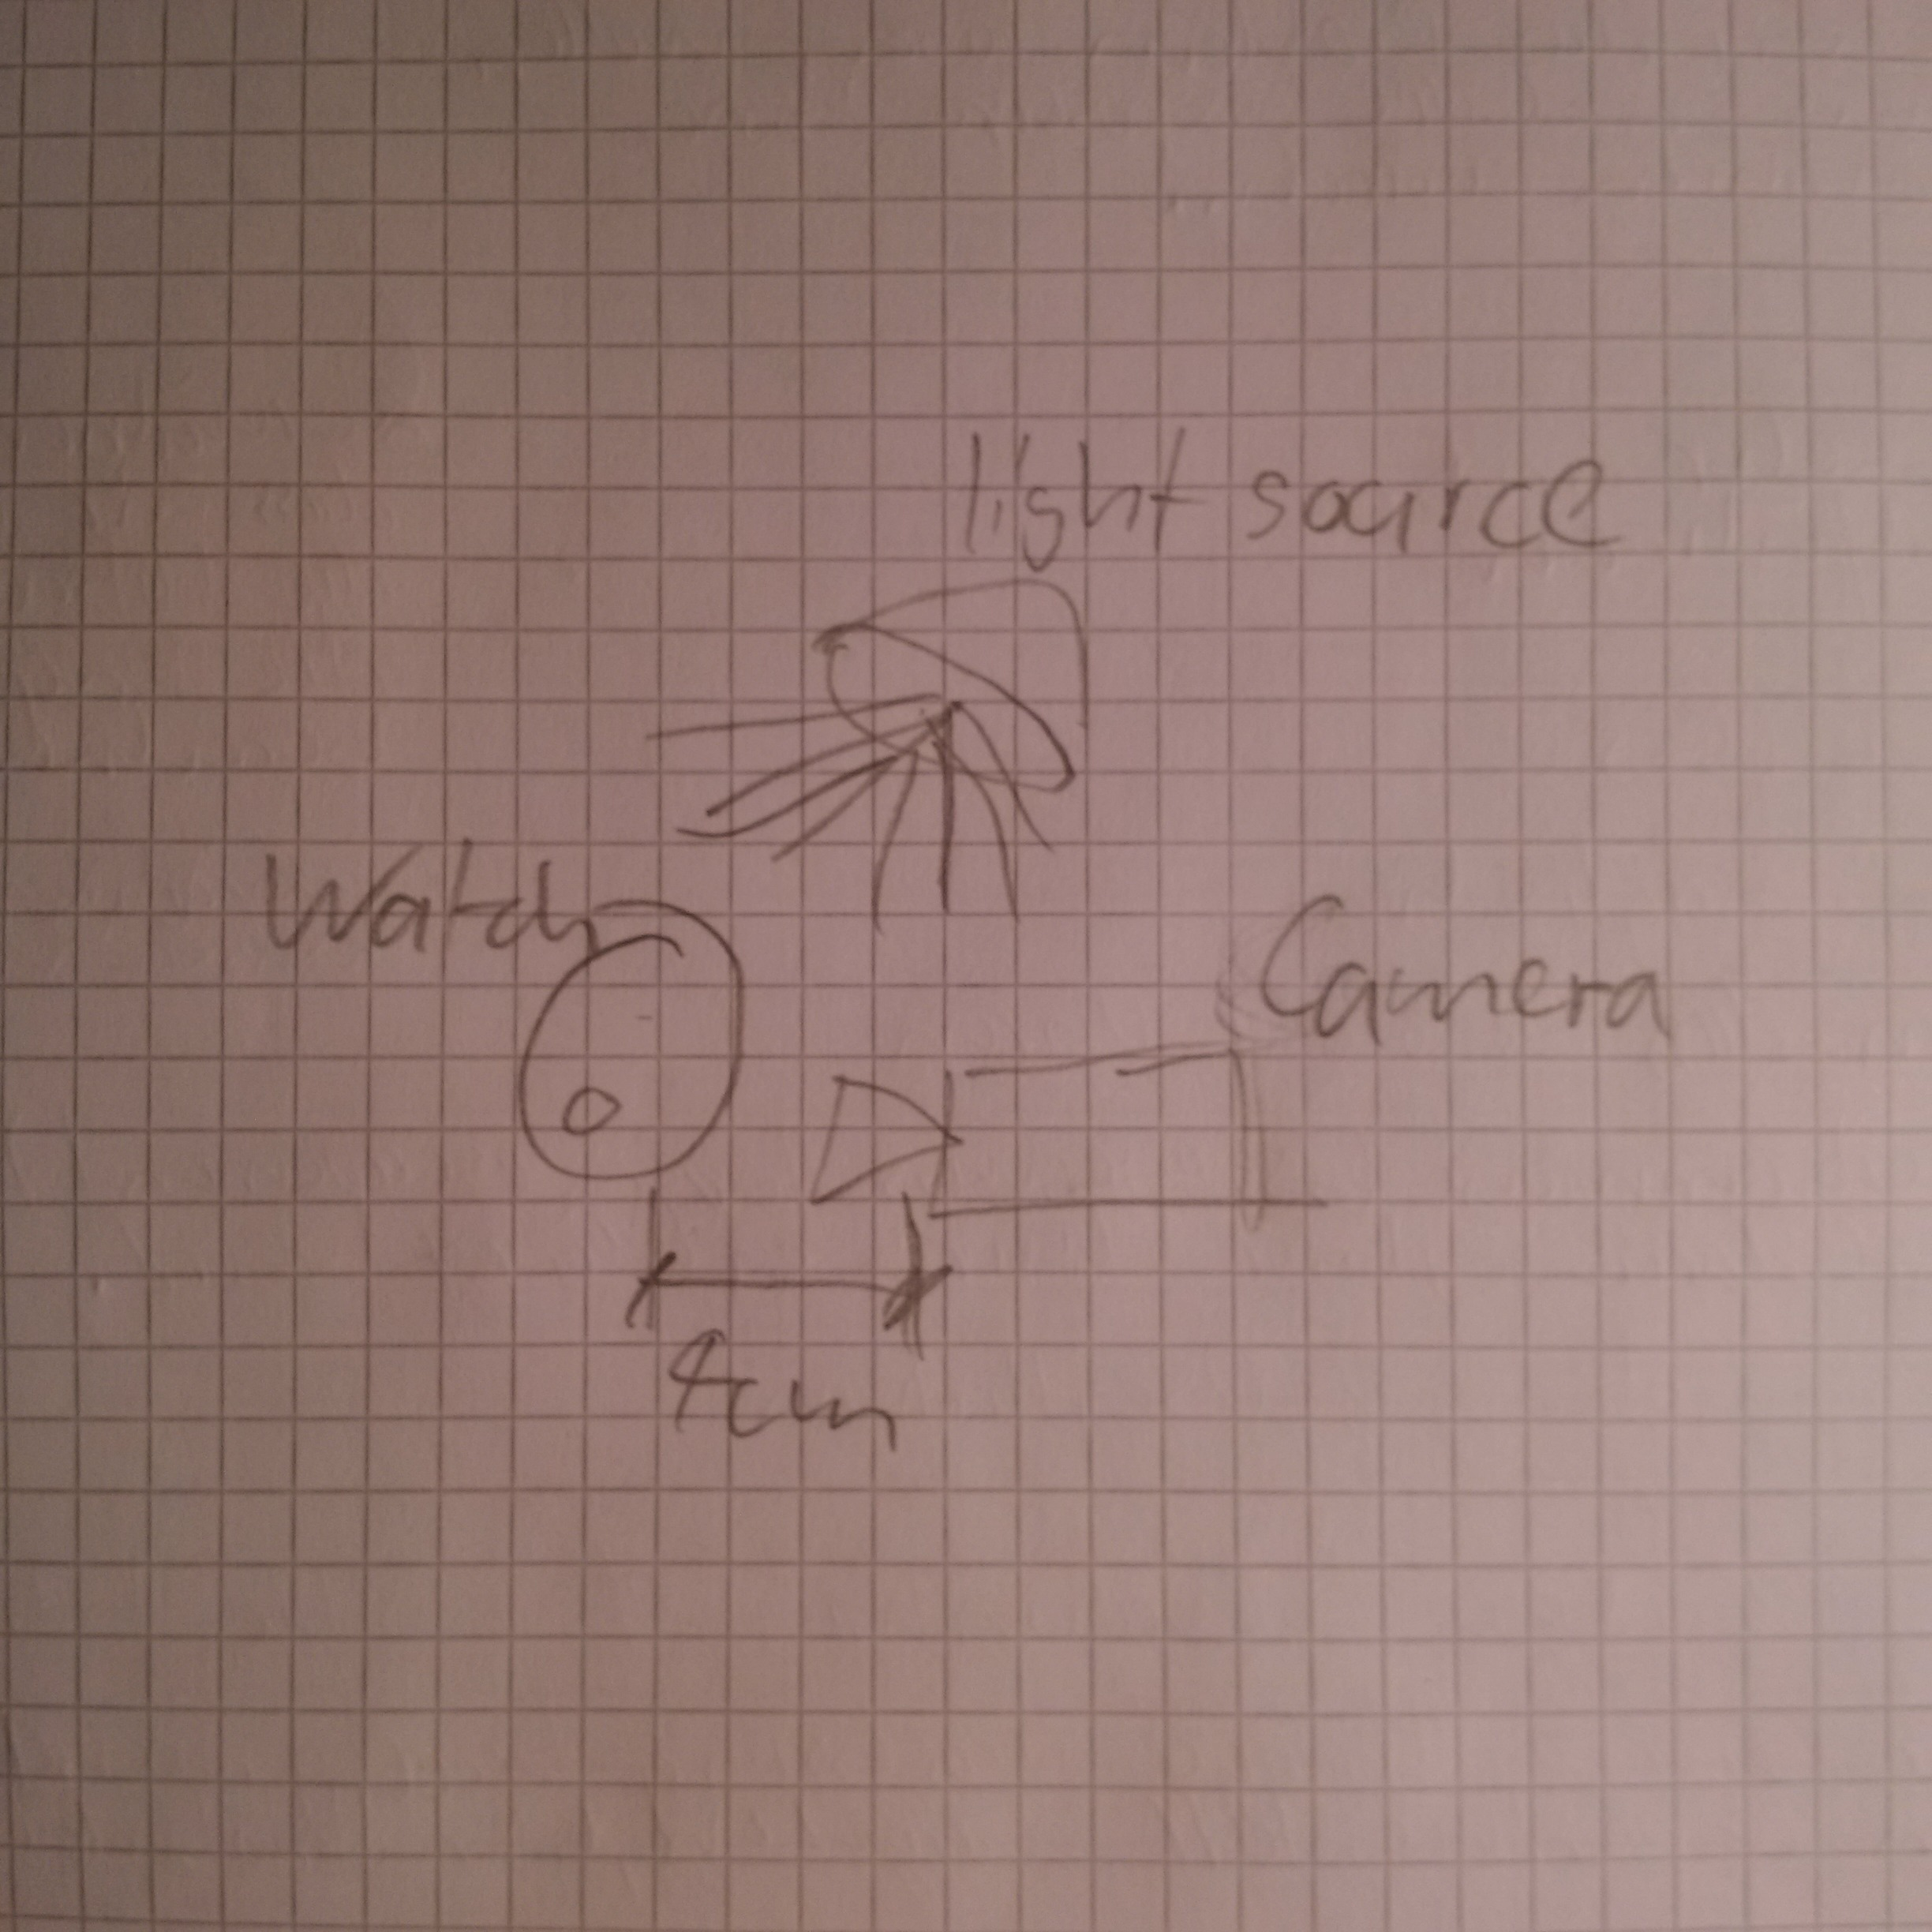
\includegraphics[scale=0.1]{Images/test_setup}
        
        \caption{Test setup for records}
        \end{figure}
        
    \section{Gesture detection}
    A first attempt was to move the hand in front of the camera down, up, right and left and to determine the direction in real time based on the motion vectors. 
    \newline
    For this, the average of all x-values and all y-values of the motion vectors of a frame are calculated and compared with a minimum value of movement that was defined. Depending on whether the x-average value is lower or higher than zero, a movement to the left or right has been detected. Likewise, it works for the y-average with the movement up or down.
        \newline
 As this worked quite well, the balance wheel of the test watch was recorded and it was tried out to detect the movement with the same program. Unfortunately, this program can only detect very clear movements. With very minimal movements this program fails, therefore the frequency of the balance wheel could not be calculated with this implementation. 
    
    \section{Animation of motion vectors}
    
    In a first step all SAD values were animated with colors to get a better understanding of how good the information they keep is and how as well as if they can be used to calculate the frequency of the movement of the balance wheel.
    
    \noindent
    \begin{figure}[H]
    \centering
    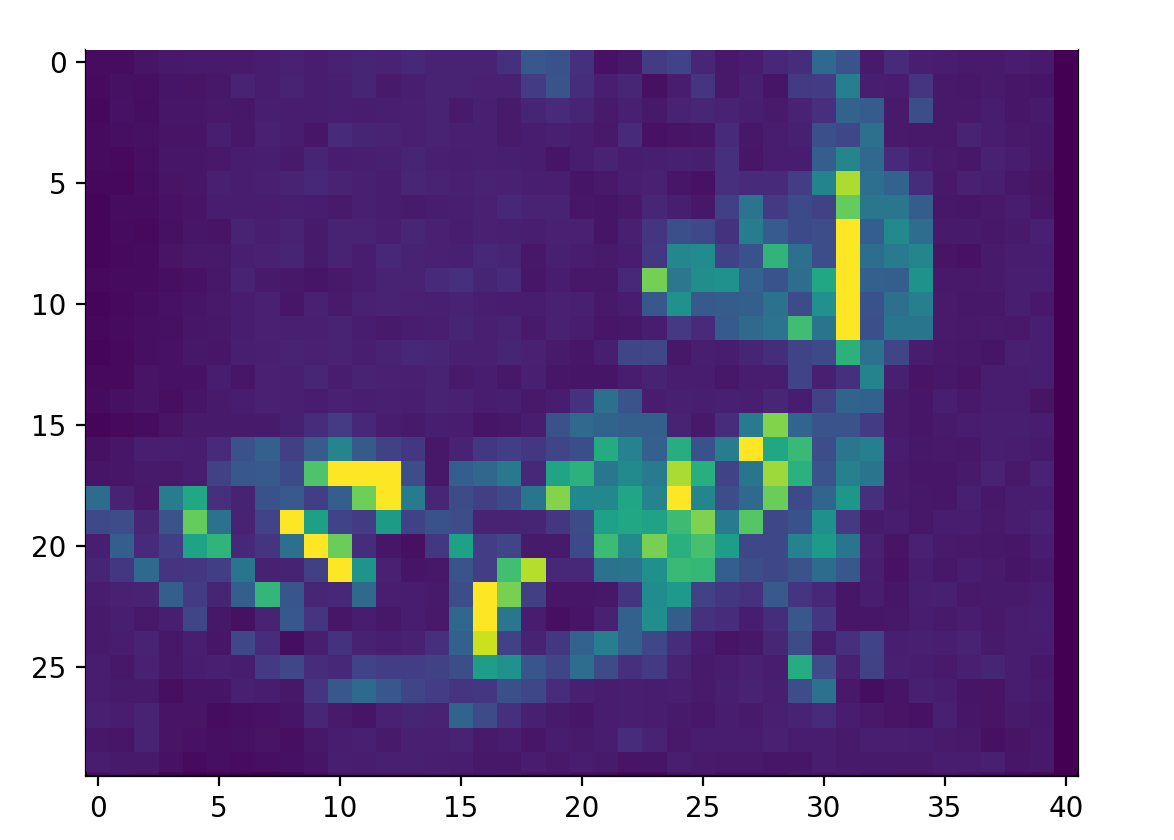
\includegraphics[scale=0.6]{Images/animation_sad.png}
    
    \caption{Snapshot of the animation of the SAD values, the lighter the color the higher the value of the SAD}
    \end{figure}
     
    Further the x and y vector were analyzed and also animated. But as those vectors itself are hard to use and only give partial information (y-vector: up or down, x-vector: right or left), the hypotenuses were calculated with Pythagoras' theorem and displayed similar to the SAD values. The hypotenuses give information about the amount as well as the direction of the motion.
    
    \noindent
    \begin{figure}[H]
    \centering
    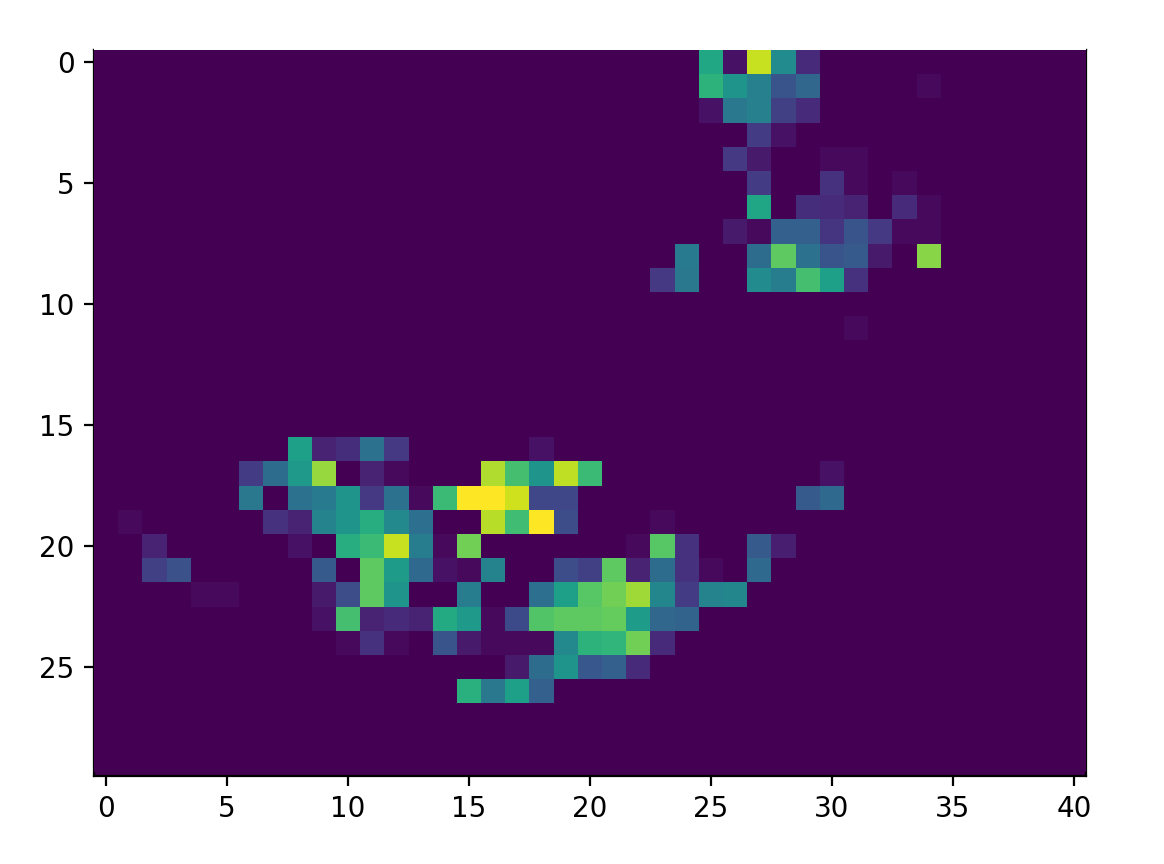
\includegraphics[scale=0.6]{Images/animation_hypotenuse.png}
    
    \caption{Snapshot of the animation of the hypotenuses, the lighter the color the higher the value of the hypotenuse}
    \end{figure}
    
    Another experimental approach was displaying the motion vectors as arrows directly in the video. This approach was helpful to get a better understanding under which conditions the best result of the motion vectors is reached.
    \pagebreak
    
    \section{Motion vectors visualized in a frame}
    Codecvisa was used to display the motion vectors of a frame.
    The result is shown in Figure 3.
 
    \noindent
    \begin{figure}[H]
    \centering
    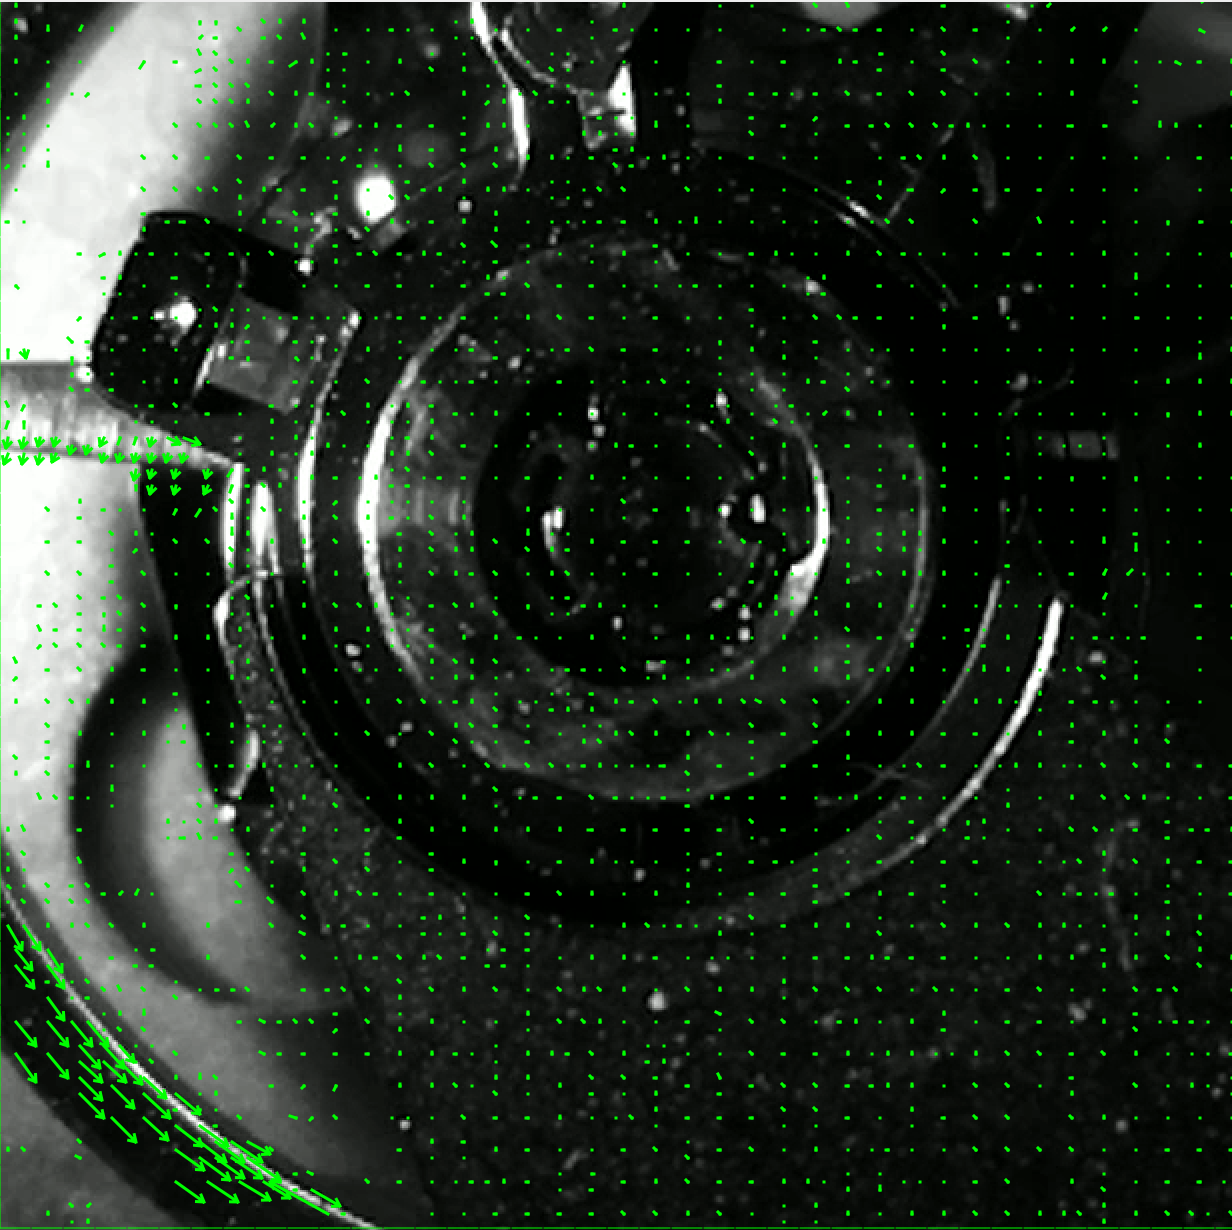
\includegraphics[scale=0.5]{Images/motion_vectors.png}
    
    \caption{Motion vectors drawn in one frame}
    \end{figure}
    
    \section{Analysis of motion vectors in excel}
    \begin{itemize}
        \item ev bild, wie das gemeint ist...
      \end{itemize}
    Another approach used Excel was to determine whether a motion vector from one frame is the predecessor of the motion vector in the next frame.
    The hope was that a moving pixel could be followed and therefore the location of the pixel would always have been known.
    The result was sobering because one frame and motion vector cannot be associated with another frame and motion vector.
    This experiment looked at the idea of the optical flux with the movement vectors of the MMAL (Multi-Media Abstraction Layer).
    
    \noindent
    \begin{figure}[H]
    \centering
    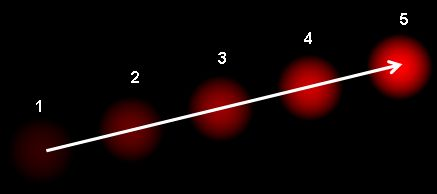
\includegraphics[scale=0.7]{Images/optical_flow_basic1.jpg}
    
    \caption{It shows a ball moving in 5 consecutive frames. The arrow shows its displacement vector.}
    \end{figure}
    
    \section{Influences of camera setup and parameters}
    Testing with different settings has shown that the results can be improved. For example, the black and white records are the better choice. Reducing the shutter speeds can reduce motion blur, which also contributes to a better result.
    The consequence of the shorter exposure time is that the light source must be very strong and close to the subject, otherwise the image is too dark and has a negative effect on the result.
    Records with changed angles were also taken. The angle was changed by about 30 degrees. With this adjustment, no significant changes in the measured values could be detected.
    Furthermore, it was recognized that the selected image detail influences the measured values. During the video recordings it was taken care that the balance wheel takes up the entire image section.
    \newpage

    \section{Crude calculation of frequency}
    With the help of the motion vectors and the corresponding time stamps per frame, a rough calculation of the frequency can be made. All x, y or SAD values contained in the image are summed up. If the sum of all values is small, it is very likely that the balance wheel is at a standstill before turning back again. For small values, the time stamp is registered and the difference to the next standstill is calculated. Since the balance wheel triggers half a oscillation, it has moved from one stop to the next half point. 
    In order to roughly calculate the frequency, an Excel sheet was created in which all the accumulated x- and y-values were entered and the standstills of the balance wheels were determined by eye. The half-oscillations and the frequency were calculated from the time intervals of the standstills. Afterwards, the average of all calculated frequencies was determined and it was recognized that the results with this method should be good enough to determine the frequency and thus the rate deviation. 
    
    \noindent
    \begin{figure}[H]
    \centering
    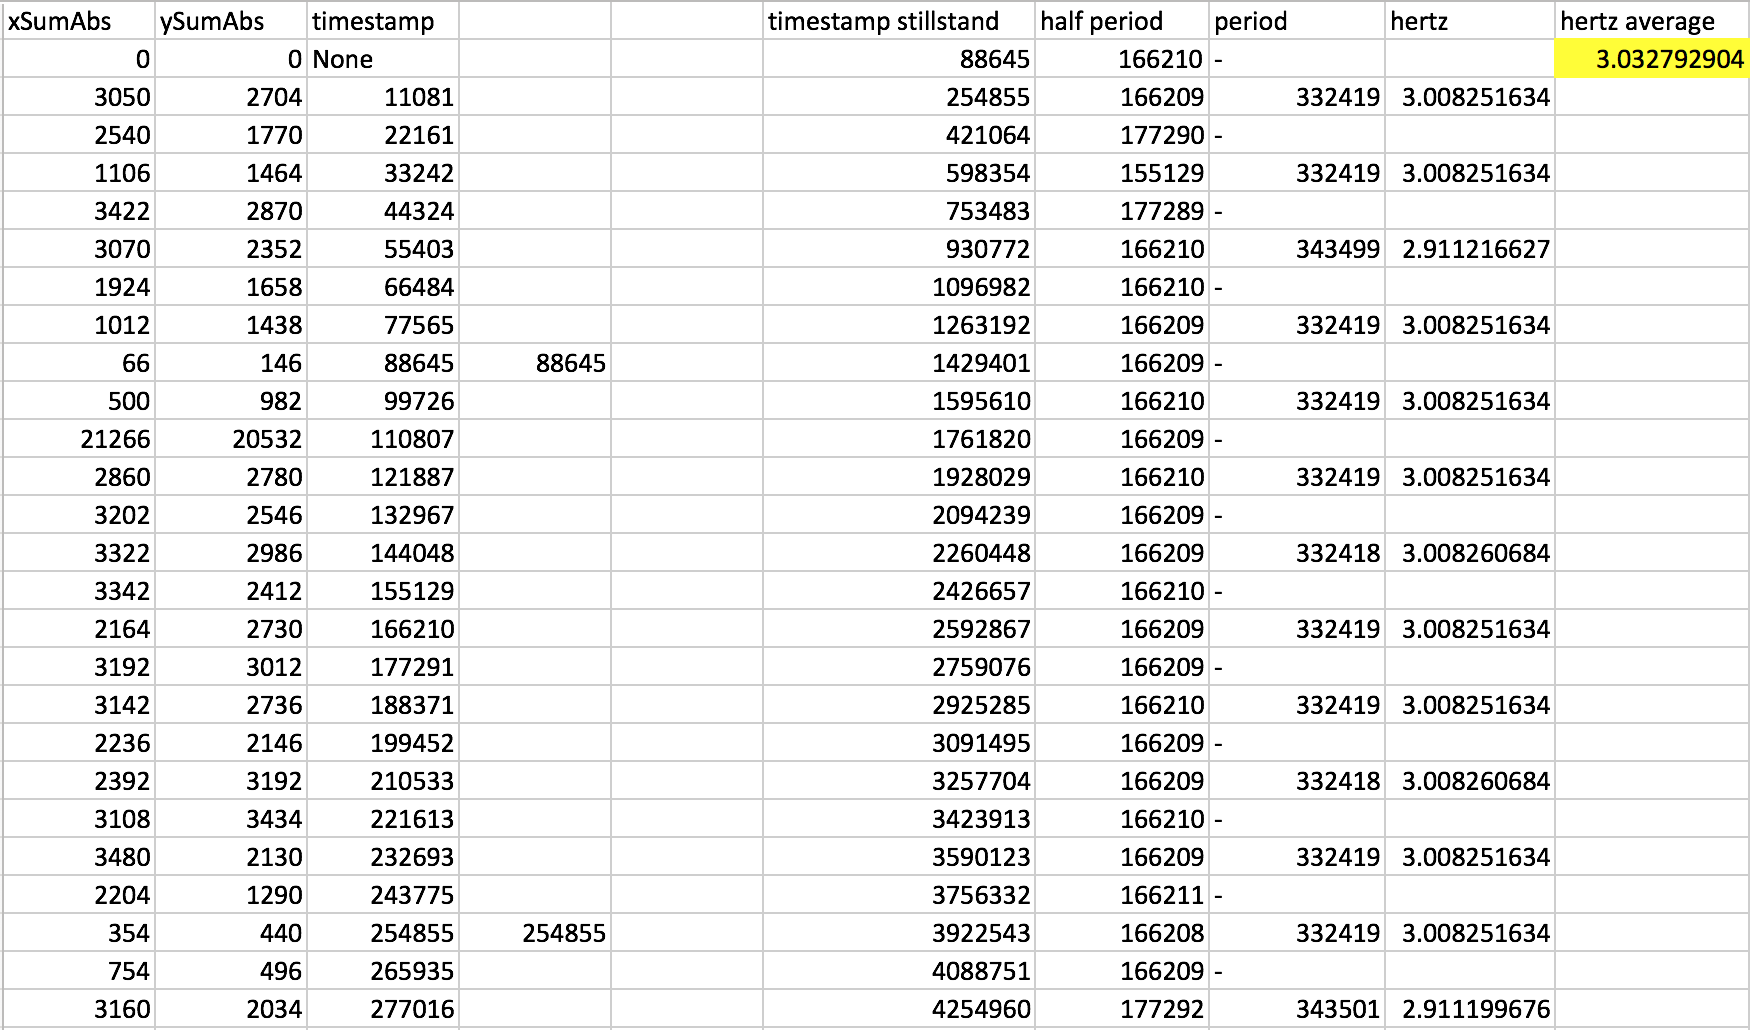
\includegraphics[scale=0.45]{Images/excel_sheet_numbers.png}
    
    \caption{Excel sheet with summed x-, y-values, timestamps and calculated frequency}
    \end{figure}

    \noindent
    \begin{figure}[H]
    \centering
    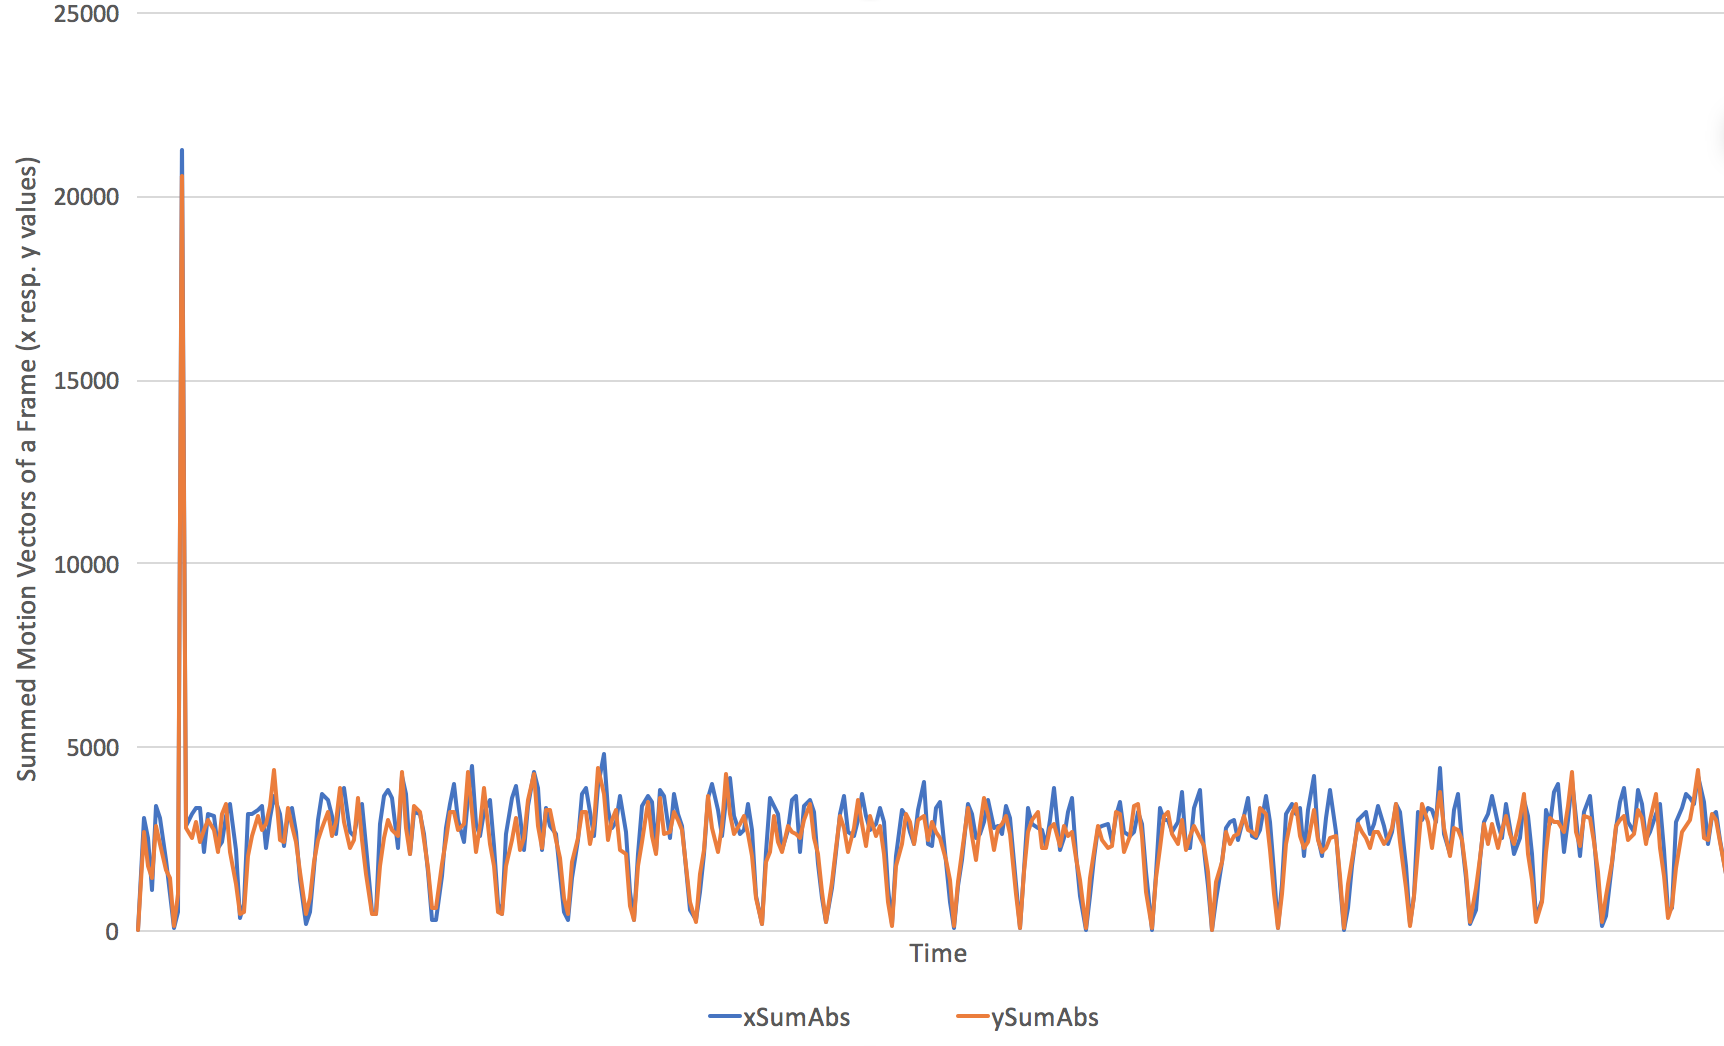
\includegraphics[scale=0.35]{Images/excel_sheet_graph.png}
    
    \caption{Illustration of summed x-(blue), y-values (red) over time. The x-axis is the time and the y-axis are the x- and y-values.}
    \end{figure}
    
    \chapter{Calculation of the frequency}
    The implementation of a Python program was based on the procedure in the rough calculation from the Excel spreadsheet. During the first implementation, it turned out that there are different methods for calculating the frequency and it resulted in three different implementations, which are explained in more detail in the following sections.
    
       \section{Implementation of the algorithms}
    \subsection{Counting minima with upper limit} 
    
    The greatest difficulty proved to be the detection of the minimia, which characterize the standstill of the balance wheel. These were relatively easy visible to the unaided eye, but in an automatic calculation, appropriate conditions had to be set in order to take into account the correct values and correct the inaccuracies caused by the image noise. The setting of an upper limit for the minima proved to be a suitable condition. All minima below this limit are therefore taken into account. 
    
    Furthermore, the calculation of the frequency in the Python program has been further simplified by not calculating each period individually, but by selecting the first and the last minimum over the whole period of time, in which it was recorded. This time span is then calculated by half of the number of minima minus 1. Half, because every half of the period the balance wheel stops and minus 1, because otherwise a half-period would be taken into account too much. This approach reduces the number of rounding errors, resulting in higher accuracy. After this calculation, the period duration T is now available, from which the frequency f can be calculated quite simply: 
    
     \begin{displaymath}
      f = \frac{1}{T}
     \end{displaymath}
     
  \subsection{Counting minima with stepsize}
  To ensure that minimas are not missed during counting, step sizes were used, that means the specifications where the minimas are to be searched for. In the measurements with the test watch, which has a stroke number of 6 per second, a frame rate of 90 was used and therefore every 15th value should show a standstill or a minimum. To detect deviations, a search window of size 5 has been defined.
  For this way, two further values are compared to the left and right of the nominal step size and 15th steps are added from the smallest value of these 5. This method does not require defining a threshold for the minima searching, which is often difficult to set. On the other hand one has to know the ideal frequency of the watch to calculate the stepsize.
  
    \subsection{Counting minima with tic toc and stepsize}
  The implementation of the program for calculating the frequency by counting the minimums with a defined step size has been adapted so that the calculation is carried out in a similar way as with the professional devices. In the previous implementation, the length of one half-period after another was measured and then the frequency calculated. However, the semi-oscillation may differ in one direction from the semi-oscillation in the other direction, so the accuracy of the program can be improved if the length is measured from one tic to the next and exactly the same for the beat on the other side, the tac, as shown in the figure below. 
       \noindent
    \begin{figure}[H]
        \centering
        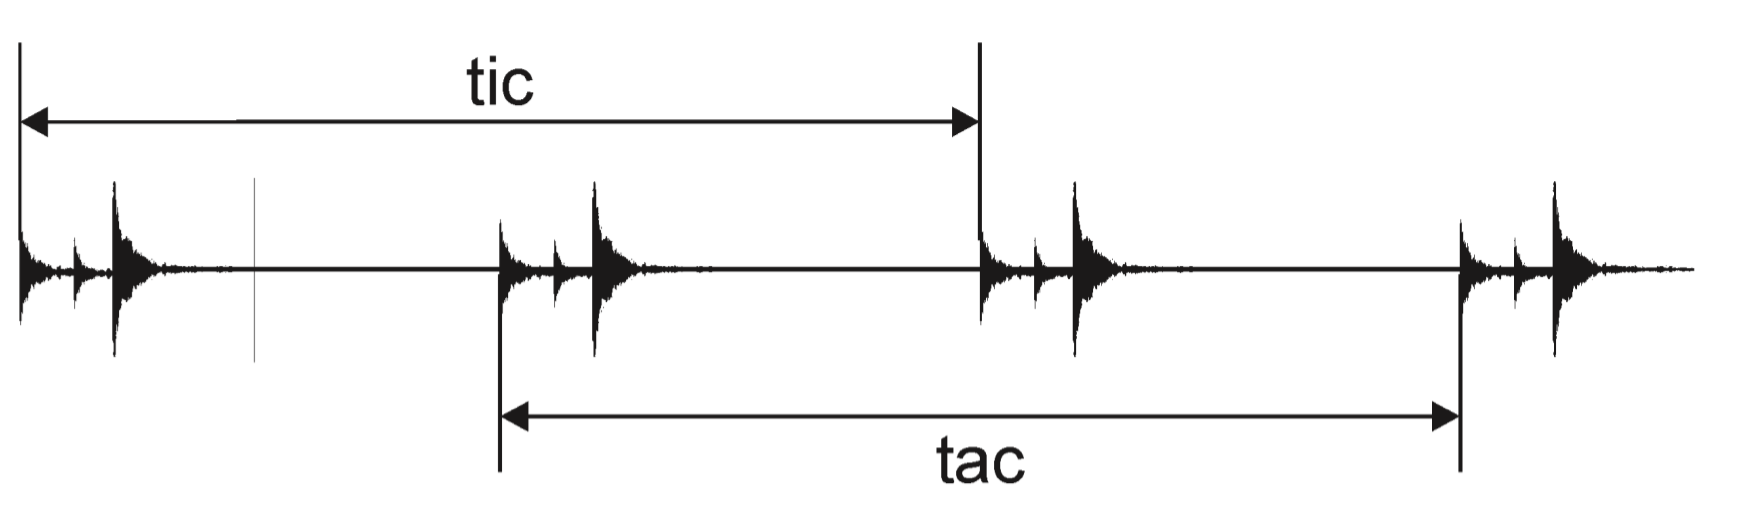
\includegraphics[scale=0.4]{Images/gangdeviation.png}
    
    \caption{Period duration of tic, resp. tac}
    \end{figure}    
  
  This results in overlapping periods, which is why the following calculation must be carried out at the end:
  
       \begin{displaymath}
     \text{period duration} = \frac{\text{period duration of tic} + \text{period duration of tac}}{2} 
     \end{displaymath}
  and therefore: 
       \begin{displaymath}
      \text{frequency}= \frac{1}{\text{period duration}}
     \end{displaymath}
     
    
    \chapter{Results}
        Reference measurements were performed on the test watch on three days. Two measurements were carried out with the Greiner Compact 900 and one with the Witschi Watch Expert II. Calculations using the Greiner Compact diverge greatly from those taken with the Watch Expert II. In the next section, this divergence and its causes will be discussed in more detail. 
    \section{Measurements}
As the test watch was in a distinctly colder environment (about 5 degrees Celsius) shortly before the Greiner Compact meter was used to measure the reference values, it is highly likely that the small metal spring has contracted and the watch ran faster as a result. Before the calculation with the Watch Expert II time scale, the test watch was in an ambient temperature of about 25 degrees Celsius for a long time. A difference of only 5 degrees Celsius can affect the accuracy of the watch. \cite{Witschi_basics} As the reference measurements are based on a difference of about 20 degrees Celsius, the above-mentioned difference occurs with the measured values obtained.
The optical measurements of the picamera were carried out on an average at about 25 degrees Celsius, therefore the reference values determined by the Wisio Scope time scale are best suited for the comparison.
\bigskip
\newline
    All measurements were taken in different positions of the watch with different length
    of recordings whereas each position was recorded in 10, 20, 40 and 80 minutes.
\bigskip
\newline
    The figure and table below show the deviation per day based on the following calculation:
    Taken the first timestamp (t1) of a stillstand and taken the last timestamp (t2) of a stillstand, the counted number of stillstands (s1), number of strokes per hour (s2 = 21600):
    \bigskip
    
    \begin{center}
    \(t2-t1 = \triangle t\)
        \bigskip
    
	\( \triangle t / s1 = \text{stroke duration}\)
	    \bigskip
    
    \((\text{stroke duration}*s2)-3600 \text{sec}=\text{deviation per hour}\)
        
    \end{center}
    
    \noindent
    \begin{figure}[H]
        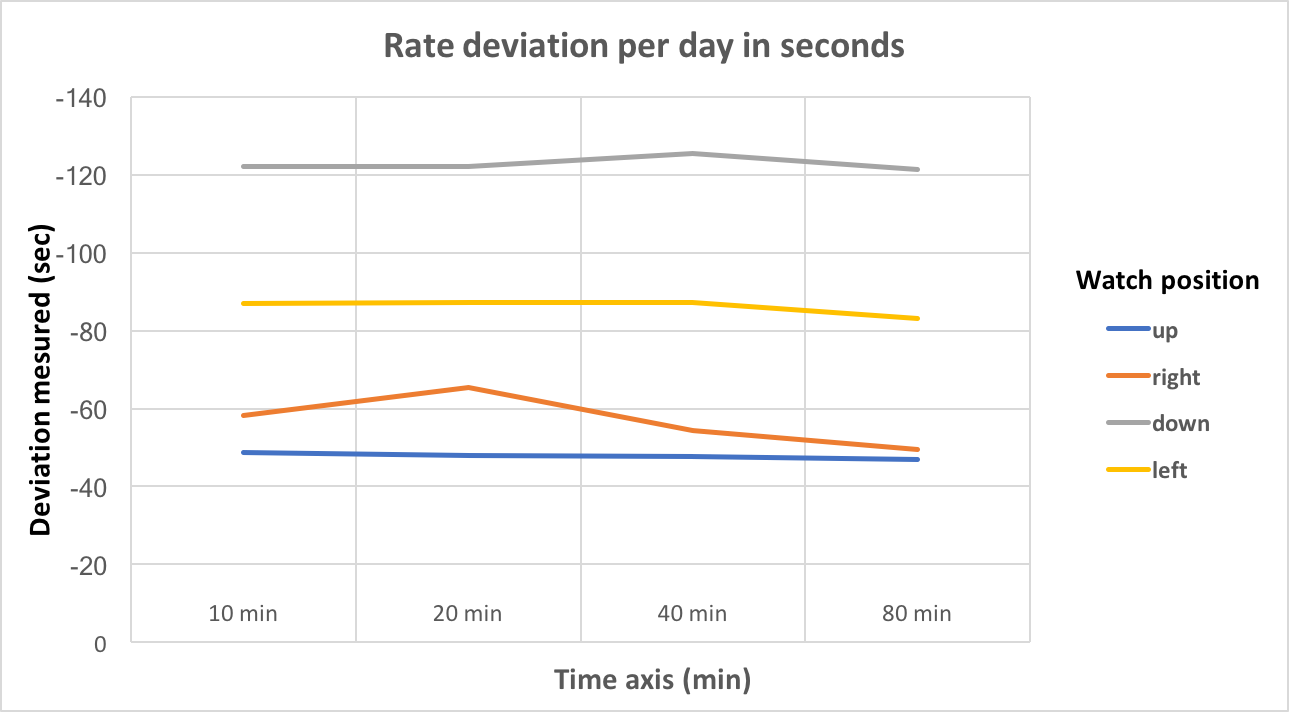
\includegraphics[scale=0.5]{Images/variations_per_day.png}
    
    \caption{ Variation of different time and position recordings}
    \end{figure}    
    
    \begin{table}[H]
      \centering
        \begin{tabularx}{\linewidth}{ |L|L|L|L|L|L|L|L|  }
        \hline
        {\fontsize{10}{12}\selectfont \textbf{Positions}} &{\fontsize{9}{10}\selectfont \textbf{Greiner Compact 900}} & {\fontsize{10}{12}\selectfont \textbf{Watch Exper II}} & {\fontsize{10}{12}\selectfont \textbf{10 min}} &  {\fontsize{10}{12}\selectfont \textbf{20 min}} &  {\fontsize{10}{12}\selectfont \textbf{40 min}} & {\fontsize{10}{12}\selectfont  \textbf{80 min}} \\ \hline
        up        & -13                 &      -31  & -48.7     & -48.0     & -47.6      & -47.0      \\ \hline
        right     & -30                 &      -64  & -58.3      & -65.5    & -54.4      & -49.4      \\ \hline
        down      & -20               &  -46  & -122.2    & -122.2     & -125.4    & -121.4      \\ \hline
        left      & -14                & -34 & -87.0	   & -87.1	  & -87.1	  & -83.1      \\ \hline
        \end{tabularx}
          \caption{ variations per day in seconds} 
    \end{table}
    
    \section{Verification of accuracy}
    The calculated frequency is far too imprecise. In theory, however, the calculation should become more precise after a certain period of time and should even be accurate to the microsecond.
    But this has never been achieved. For this reason, a reliable artificial clock was used in the form of an LED that is clocked by a 50 Mhz quartz and is therefore sufficiently accurate.
    
    Because trust in the motion vectors has diminished, a color-based method was used. The new method analyzes certain pixels in each image of the video sequence and detects the LED's light when a threshold value is exceeded in the RGB color space.
    The LED has been programmed to mimic the test watch's balance wheel and provide 21600 pulses per hour -
    respectively a frequency of 3 Hz.

    The measurement is already accurate to approx. 7 microseconds at 60 seconds, as can be seen in the table below.

    \begin{itemize}
      \item Grafik von Excel wo man sehen kann, dass die Messung nicht besser wird, weil es Messfehler gibt, die nicht erklärt werden können.
      \item statistic table hinzufügen
    \item als schlusswort: Messungen mit Kamera sind genau genug
    \end{itemize}
   
    \begin{table}[H]
      \centering
        \begin{tabularx}{\linewidth}{ |L|L|L|L|L|L|  }
        \hline
        \textbf{Duration} [s] &  \textbf{run 1}  [\si\micro\/s]&  \textbf{run 2} [\si\micro\/s]&  \textbf{run 3} [\si\micro\/s]&  \textbf{run 4} [\si\micro\/s]&  \textbf{run 5} [\si\micro\/s]\\ \hline
        10        & 166591.5                 & 166585.0     & 166397.2     & 165655.4      & 166585.0      \\ \hline
        20     & 166679.0                 & 166117.1      & 166675.0    & 166675.0      & 166581.9  \\ \hline
        40      & 166486.4                 & 166673.1    & 166675.0     & 166440.3    & 166673.1    \\ \hline
        60      & 166673.7                 & 166672.4	   & 166673.7	  & 166672.4	  & 166673.7  \\ \hline
        300      & 166665.2                 & 166671.7	   & 166640.4	  & 166665.3	  & 166640.4      \\ \hline
        600      & 166668.2                 & 166649.6	   & 166668.2	  & 166655.8	  & 166668.2      \\ \hline
        900      & 166667.2                 & 166667.3	   & 166638.4	  & 166638.4	  & 166667.2      \\ \hline
        1200      & 166660.4                 & 166668.3	   & 166669.7	  & 166668.2	  & 166668.2      \\ \hline
        1500      & 166668.8                 & 166650.3	   & 166650.3	  & 166668.8	  & 166668.8      \\ \hline
        1800      & 166652.8                 & 166668.2	   & 166669.2	  & 166668.2	  & 166669.2      \\ \hline
        2100      & 166668.6                 & 166668.6	   & 166668.6	  & 166655.4	  & 166654.5      \\ \hline
        2400      & 166668.1                 & 166652.7	   & 166656.5	  & 166668.1	  & 166668.1        \\ \hline
    \end{tabularx}
    \caption{Measured half periods of led board using RGB values of pixels. Desired value 166666}
    \end{table}

    \begin{table}[H]
      \centering
        \begin{tabularx}{\linewidth}{ |L|L|L|L|L|L|  }
        \hline
        \textbf{Duration} [s] &  \textbf{run 1}  [\si\micro\/s]&  \textbf{run 2} [\si\micro\/s]&  \textbf{run 3} [\si\micro\/s]&  \textbf{run 4} [\si\micro\/s]&  \textbf{run 5} [\si\micro\/s]\\ \hline
        10        & 166636.1                 & 166628.1     & 166628.1     & 166628.1      & 166628.1      \\ \hline
        20     & 166700.3                 & 166602.3      & 166700.3    & 166602.3     & 166602.3  \\ \hline
        40      & 166685.6                 & 166638.1    & 166638.1     & 166638.1    & 166638.1    \\ \hline
        60      & 166649.5                 & 166649.5	   & 166649.5	  & 166649.5	  & 166649.5  \\ \hline
        300      & 166667.4                 & 166667.4	   & 166673.6	  & 166667.4	  & 166667.4      \\ \hline
        600      & 166666.5                 & 166666.5	   & 166666.5	  & 166669.6	  & 166666.5      \\ \hline
        900      & 166668.2                 & 166666.2	   & 166668.3	  & 166668.3	  & 166651.7      \\ \hline
        1200      & 166669.1                 & 166656.7	   & 166658.3	  & 166658.4	  & 166669.3      \\ \hline
        1500      & 166669.7                 & 166659.8	   & 166658.5	  & 166669.6	  & 166659.7      \\ \hline
        1800      & 166661.7                 & 166660.7	   & 166668.9	  & 166669.9	  & 166668.9      \\ \hline
        2100      & 166668.4                 & 166661.4	   & 166668.4	  & 166669.3	  & 166662.3      \\ \hline
        2400      & 166669.7                 & 166669.6	   & 166663.5	  & 166663.5	  & 166662.7        \\ \hline
    \end{tabularx}
    \caption{Measured half periods of led board using motion vectors. Desired value 166666}
    \end{table}
    
    \chapter{Discussion}
    With the help of the picamera library and motion vectors the frequency of the balance of a mechanical watch was calculated with different implementations. Overall, the frequency was determined relatively accurate and without large deviations. Actually, all methods worked, but the implementation with the step size and the consideration of the direction of the semi-oscillation did best. If more research is done, such as whether and how to improve the camera settings, the results could possibly be further improved. 
    
    \section{Difficulties}
    \begin{itemize}
    \item Kameraeinstellungen und Lichverhältnisse finden
    \item schwer gute Referenzmessungen zu bekommen
    \item Zuerst zu viele Informationen abgespeichert -> zu wenig speicher
    \end{itemize}
    
    \section{Outlook}
    In this work it was shown that with relatively inexpensive hardware, sufficient good measurements can be carried out to determine the accuracy of a watch. Compared to the professional equipment, which costs thousands of dollars to buy, a good user interface could create a product that is much cheaper and can still keep up with the measurements of more expensive devices. 
    
    \glsaddall
    \printglossaries

\addcontentsline{toc}{chapter}{Bibliography}
\printbibliography
        
    \addcontentsline{toc}{chapter}{List of Figures}    
    \listoffigures
    \bigskip
      
    \addcontentsline{toc}{chapter}{Appendix - Python programs}
     \chapter*{Appendix - Python programs}  
     \section*{searchMinima\_tic\_toc.py}  
      \lstset{
       basicstyle=\fontsize{10}{12}\selectfont\ttfamily,
           keywordstyle=\color{blue}\ttfamily,
           stringstyle=\color{red}\ttfamily,
           commentstyle=\color{teal}\ttfamily,
          breaklines=true
          }  
    \lstinputlisting[language=Python]{Files/searchMinima_tic_toc.py}
    
    \end{document}